\chapter{Basis Transformationen }
\label{sec:basisTransformation} 





 
In den folgenden Kapiteln werden zunächst ein paar Grundlegende mathematische Operationen vorgestellt, welche das Grundgerüst der Stereokalibrierung und Szenenrekonstruktion bilden.
%Um die mathematischen Vorgehensweisen dieser Arbeit verständlicher zu machen, werden in den folgenden Kapiteln zunächst ein paar Grundlegende mathematische Operationen vorgestellt, welche das Grundgerüst der Stereokalibrierung und Szenenrekonstruktion bilden. 
Als aller erstes werden anhand praxisnaher Beispiele die Notwenidigkeit der Basis Transformation und damit einhergehend der Spezialfall einer Transformation von einem Koordinatensystem wie zum Beispiel einem Weltkoordiantensystem $(O,\delta)$ mit $\delta=(d_1, d_2, d_3)$ in ein Kamerakoordinatensystem $(C,\beta)$ mit $\beta=(b_1,b_2,b_3)$ aufgezeigt. Noch anzumerken ist, dass in dieser Arbeit grundlegend von orthogonalen Koordinatensystemen ausgegangen wird, andernfalls wird explizit darauf hingewiesen. 



%\section{Die Transformation von Koordinaten schließt die Transformation der Basis mit ein}
%
%Es sei \textit{V} ein \textit{n}-Dimensionaler Vektorraum über einem Körper \textit{K}. \textit{K} stellt in diesem Beispiel das Skalar \ensuremath{\mathbb{R}} dar, welches alle reelen Zahlen mit einschließt. Zur Veranschaulichung wird der Vektorraum  \ensuremath{V^3} also ein 3-Dimesnionaler Raum gewählt, dessen Basis mit \ensuremath{\beta = [\vec{b}_1, \vec{b}_3, \vec{b}_3]} bezeichnet wird.\cite{Elements} ....  (FORTFÜHREN)\\
%
%A vector $\vec{v} \in V^3$ is uniquely expressed as a linear combination of basic vectors of V 3 by its coordinates $(x,y,z) \in \mathbb{R}$. $\vec{v} = xb_1+yb_2+zb_3$ and can be represented as an ordered triple of coordinates, $\vec{v}_\beta =[x\,y\,z]^T$

\section{Koordinatentransformation durch Basistransformationen}

Anhand eines Beispiels wird die Transformation der Koordinaten noch genauer veranschaulicht. Es soll kompakt in einer Symbolischen Schreibweise Punkte aus einem Weltkoordinatensystem  
$(O,\delta)$ mit $\delta = (d_1,d_2,d_3)$ in ein Kamerakoordinatensystem  $(C,\beta)$ mit $\beta = (b_1,b_2,b_3)$ überführt werden, welches eine Verschiebung und Rotation zum Weltkoordinatesystem aufweist. Beispielhaft wird dies in Abbildung \ref{fig:Koordinatensysteme1} aufgezeigt.
 
	\begin{minipage}{\linewidth}
		\centering
		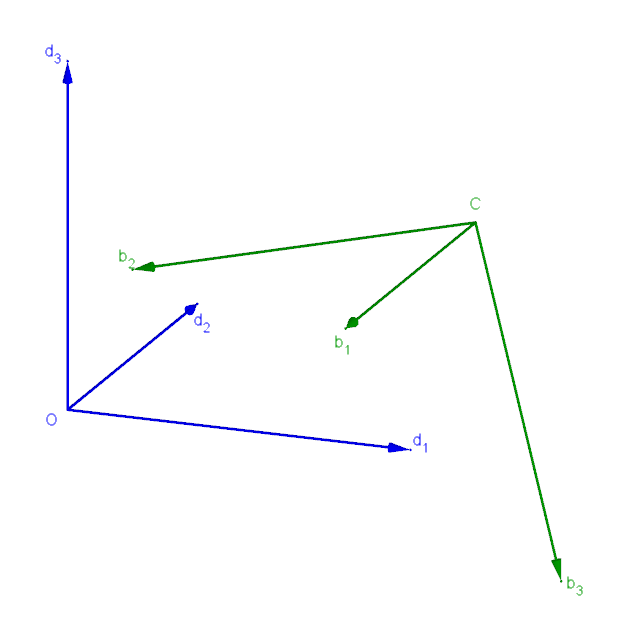
\includegraphics[width=0.6\linewidth]{images/WeltKordSys.png}
		\captionof{figure}{Weltkoordinatensystem $(O,\delta)$ mit $\delta = (d_1,d_2,d_3)$ und Kamerakoordinatensystem  $(C,\beta)$ mit $\beta = (b_1,b_2,b_3)$ }
		\label{fig:Koordinatensysteme1}
	\end{minipage}\\ \\
	
	
Zunächst wird eine sogenannte Koordinatisierung von Punkten im Weltkoordinatensystem vorgenommen. Ein Punkt $P_\delta$ bezüglich des Weltkoordinatensystems wird dann wie folgt beschrieben.

	
	\begin{gather}
	P_\delta = O + p_{1\delta}d_1 + p_{2\delta}d_2 + p_{3\delta}d_3\\
	\leadsto P_\delta = (p_{1\delta},p_{2\delta},p_{3\delta})^T = \begin{pmatrix} p_{1\delta} \\ p_{2\delta} \\ p_{3\delta} \end{pmatrix}
	\end{gather}
	
	Dieses Koordinatentupel wird dann zum Zweck der Einführung homogener Objekte projektiv Erweitert.
	
	\begin{gather}
	P_\delta = \begin{bmatrix} p_{1\delta} \\ p_{2\delta} \\ p_{3\delta} \\1 \end{bmatrix} = \left\{ k \begin{bmatrix} p_{1\delta}\\p_{2\delta}\\p_{3\delta}\\1 \end{bmatrix} \in \mathbb{R} ^4 |  k \in \mathbb{R}\right\}\\
	\begin{bmatrix}\lambda p_{1\delta}\\ \lambda p_{2\delta} \\ \lambda p_{3\delta} \\ 1 \end{bmatrix} = \begin{bmatrix}p_{1\delta} \\ p_{2\delta} \\ p_{3\delta} \\ 1\end{bmatrix} \text{für} \; \lambda \ne 0
	\end{gather}

	
	Ein Punkt $P_\beta$ bezüglich des Kamerakoordinatensystem wird im Vergleich wie folgt beschrieben.
	
	\begin{gather}
	P_\beta = C + p_{1\beta}b_1 + p_{2\beta}b_2 +  p_{3\beta}b_3\\
	P_\beta = \begin{pmatrix} p_{1\beta} \\  p_{2\beta} \\ p_{2\beta}\end{pmatrix}
	\end{gather}\\
	
	Zwischen den beiden Koordinatensystemen	$(O,\delta)$  und $(C,\beta)$ werden die folgenden Beziehungsgleichungen aufgestellt. 
	
	\begin{gather}
	C_\beta = O_\delta + C_{\beta,1}d_1 +C_{\beta,2}d_2 + C_{\beta,3}d_3\\
	b_1 = (b_1)_1d_1 +  (b_1)_2d_2 +  (b_1)_3d_3\\
	b_2 = (b_2)_1d_1 +  (b_2)_2d_2 +  (b_2)_3d_3\\
	b_3 = (b_3)_1d_1 +  (b_3)_2d_2 +  (b_3)_3d_3
	\end{gather}
	
	Diese Beziehungsgleichungen können nun in Gleichung 2.1 eingesetzt werden.
	
	\begin{gather}
	\begin{split}
	P_\delta = O + (C_{\beta,1} + p_{1\beta}(b_1)_1 +  p_{2\beta}(b_2)_1 + p_{3\beta}(b_3)_1) \cdot d_1\\
	+(C_{\beta,2} + p_{1\beta}(b_1)_2 +  p_{2\beta}(b_2)_2 + p_{3\beta}(b_3)_2) \cdot d_2\\
	+ (C_{\beta,3} + p_{1\beta}(b_1)_3 +  p_{2\beta}(b_2)_3 + p_{3\beta}(b_3)_3) \cdot d_3
	\end{split}
	\end{gather}
	
Aus Gleichung 2.11 wird ein Gleichungssystem aufgestellt und gelöst.
	
	\begin{gather}
	\begin{split}
	p_{1\delta} = C_{\beta,1} + (C_{\beta,1} + p_{1\beta}(b_1)_1 +  p_{2\beta}(b_2)_1 + p_{3\beta}(b_3)_1) \\
	\leadsto \: p_{1\delta} - C_{\beta,1} =  (C_{\beta,1} + p_{1\beta}(b_1)_1 +  p_{2\beta}(b_2)_1 + p_{3\beta}(b_3)_1)
	\end{split}
	\end{gather}
	
Wenn $P_\beta$ gegeben ist, erhält man auf diese Weise direkt $P_\delta$. Wenn jedoch  $P_\delta$  gegeben ist, so muss das LGS aufgestellt und gelöst werden.
	
	\begin{gather}
	\begin{bmatrix}(b_1)_1 & (b_2)_1 & (b_3)_1\\
	(b_1)_2 & (b_2)_2 & (b_3)_2\\
	(b_1)_3 & (b_2)_3 & (b_3)_3
	\end{bmatrix} 
	\begin{pmatrix}
	p_{1\beta}\\p_{2\beta}\\ p_{3\beta}
	\end{pmatrix} = 
	\begin{pmatrix}
	p_{1\delta} - C_{\beta,1}\\
	p_{2\delta} - C_{\beta,2}\\
	p_{3\delta} - C_{\beta,3}
	\end{pmatrix}
	\end{gather}
	
 Wenn $(C,\beta)$ ein kartesisches Koordinatensystem ist, so ist die entstehende  koeffizientenmatrix $M_\beta$ orthogonal und es gilt \ensuremath{M_\beta^{-1} = M_\beta^T}. 
	\begin{gather}
	M_\beta^{T} = 
	\begin{bmatrix}(b_1)_1 & (b_1)_2 & (b_1)_3\\
	(b_2)_1 & (b_2)_2 & (b_2)_3\\
	(b_3)_1 & (b_3)_2 & (b_3)_3
	\end{bmatrix} \\
	\begin{split}
	\leadsto \: \begin{pmatrix}
	p_{1\beta}\\p_{2\beta}\\ p_{3\beta}
	\end{pmatrix}
	= M_\beta^T 
	\begin{pmatrix}
	p_{1\delta} - C_{\beta,1}\\
	p_{2\delta} - C_{\beta,2}\\
	p_{3\delta} - C_{\beta,3}
	\end{pmatrix}
	\end{split} 
	\end{gather}
	
Handelt es sich um kein kartesisches Koordinatensystem, so muss lediglich die Inverse \ensuremath{M_\beta^{-1}} anstatt \ensuremath{M_\beta^T} gebildet und wie gehabt verfahren werden. Im Folgenden wird noch einmal kompakt und in einer symbolischen Schreibweise die Transformation von Welt- in Kamerakoordinaten  festgehalten. Einmal wird wie bereits angefangen mit Spaltenvektoren gearbeitet, das selbe Verfahren wird dann noch einmal mit Zeilenvektoren dargestellt. Beide Ansätze funktionieren nach dem selben Prinzip, nur dass sich die Darstellung der Matrizen ändert. Es ist jedoch gerade wenn man mit Programmen wie Beispielsweise \textit{Matlab} arbeitet wichtig zu wissen welche Darstellung benutzt wird und worin sie sich unterscheiden. Auf diese weise passieren keine Fehler beim Interpretieren der späteren Resultate. \textit{MatLab} arbeitet beispielsweise mit Spaltenvektoren, während im entstandenen Algorithmus dieser Arbeit mit Zeilenvektoren gearbeitet wurde. Zur Erinnerung, es gilt, dass $(\beta = (b_1,b_2,b_3))$ durch Rotation $R$ aus $\delta = (d_1,d_2,d_3)$ entstanden ist.
Da es sich aber in einem nicht-kartesischen Koordinatensystem nicht um eine orthogonale Drehmatrix handelt wird die Rotation \textit{R} in diesem Beispiel als Transformationsmatrix \textit{C} gekennzeichnet. Somit soll gekennzeichnet werden, dass die Transformation unabhängig der Definition ihres ausgehenden Koordinatensystem allgemein formuliert werden kann. Es gilt für die Transformation von Welt- in Kamerakoordinaten ausgehend von Spaltenvektoren folgendes.
	
	\begin{gather}
	\begin{pmatrix}
	b_1\\
	b_2\\
	b_3\\
	C_\beta
	\end{pmatrix} = 
	\begin{bmatrix}
	c_{11} & c_{21} & c_{31} & 0\\
	c_{12} & c_{22} & c_{32} & 0\\
	c_{13} & c_{23} & c_{33} & 0\\
	C_{\beta,1} & C_{\beta,2} & C_{\beta,3} & 1
	\end{bmatrix}
	\begin{pmatrix}
	d_1\\
	d_2\\
	d_3\\
	O_\delta
	\end{pmatrix}\\
	C^T = C^{-1}= \begin{bmatrix}
	c_{11} & c_{12} & c_{13} \\
	c_{21} & c_{22} & c_{23} \\
	c_{31} & c_{32} & c_{33} 
	\end{bmatrix}\\
	C = \begin{bmatrix}
	c_{11} & c_{21} & c_{31} \\
	c_{12} & c_{22} & c_{32} \\
	c_{13} & c_{23} & c_{33} 
	\end{bmatrix}
	\end{gather}

Dementsprechend muss für die Rücktransformation von Kamera in Weltkoordinaten nur wieder die transformierte beziehungsweise die Inverse \ensuremath{C^{-1}} gebildet werden. Des Weiteren muss der Verschiebungsvektor ebenfalls mit dieser Inversen Mulitpliziert werden, um diesen ebenfalls in das Zielkoordinatensystem zu überführen.
	
	
	\begin{gather}
	\leadsto \: \begin{pmatrix}
	d_1\\
	d_2\\
	d_3\\
	O_\delta
	\end{pmatrix} = 
	\begin{bmatrix}
	c_{11} & c_{21} & c_{31} & 0\\
	c_{12} & c_{22} & c_{32} & 0\\
	c_{13} & c_{23} & c_{33} & 0\\
	&-(	C_{\beta,1}, C_{\beta,2}, C_{\beta,3})C^{-1}& & 1
	\end{bmatrix}
	\begin{pmatrix}
	b_1\\
	b_2\\
	b_3\\
	C_\beta
	\end{pmatrix}
	\end{gather}
	
	
	
	
%	Die  Rücktransformation von Kamera- in Weltkoordinaten beinhaltet mit Spaltenvektoren dargestellt also folgendes:
%	
%	\begin{gather}
%	(a,b,c,1) 
%	\begin{bmatrix}
%	c_{11} & c_{12} & c_{13} & 0\\
%	c_{21} & c_{22} & c_{23} & 0\\
%	c_{31} & c_{32} & c_{33} & 0\\
%	o_{c,1} & o_{c,2} & o_{c,3} & 1
%	\end{bmatrix}
%	= (0,0,0,1)
%	\end{gather}
	
	Die Formel 2.21 zeigt die selbe Transformation nur werden die Koordinatensysteme als Zeilenvektoren dargestellt.

	\begin{gather}
	(b_1, b_2, b_3, C_\beta) = (d_1,d_2, d_3, O) \cdot
	\begin{bmatrix} 
	c_{11} & c_{21} & c_{31} & C_{\beta,1}\\
	c_{12} & c_{22} & c_{23} & C_{\beta,2}\\
	c_{13} & c_{32} & c_{33} & C_{\beta,2}\\
	0           &       0       &   0         & 1   
	\end{bmatrix}
	\end{gather}	
	
	Daraus folgt, dass für den Fall der Rücktransformation gilt:
	
	\begin{gather}
	\leadsto \: \begin{pmatrix}
	d_1,d_2,d_3,O
	\end{pmatrix} = 
	\begin{bmatrix}
	c_{11} & c_{12} & c_{13} & \\
	c_{21} & c_{22} & c_{23} &  -\begin{pmatrix}
C_{\beta,1}\\
C_{\beta,2}\\
C_{\beta,3}
	\end{pmatrix}C^{-1}\\
	c_{31} & c_{32} & c_{33} & \\
	0&0&0 & 1
	\end{bmatrix}
	\begin{pmatrix}
	b_1,b_2,b_3,C_\beta
	\end{pmatrix}
	\end{gather}
	
 Als Zwischenfazit lässt sich festhalten, dass sich die Matrix zur Beschreibung der Koordinatentransformation aus \textit{C} und einem Spalten- beziehungsweise Zeilenvektor der Form  \ensuremath{\vec{v}=\begin{pmatrix}
		C_{\beta,1}\\C_{\beta,2}\\C_{\beta,3}\\
	\end{pmatrix}} oder \ensuremath{\vec{v}=\begin{pmatrix}
	C_{\beta,1}&C_{\beta,2}&C_{\beta,3}\\
\end{pmatrix}} zusammensetzt.

\begin{gather}
		\begin{bmatrix}
	c_{11} & c_{21} & c_{31} & 0\\
	c_{12} & c_{22} & c_{32} & 0\\
	c_{13} & c_{23} & c_{33} & 0\\
	&-(C_{\beta,1}, C_{\beta,2}, C_{\beta,3})C^{-1}& & 1
	\end{bmatrix}\\
		\begin{bmatrix}
	c_{11} & c_{21} & c_{31} & \\
	c_{12} & c_{22} & c_{32} & -\begin{pmatrix}
	C_{\beta,1}\\C_{\beta,1}\\ C_{\beta,1}
	\end{pmatrix}C^{-1}\\
	c_{13} & c_{23} & c_{33} &\\
	0&0&0&1
	\end{bmatrix}
\end{gather}\\

Da im implementierten Code dieser Arbeit mit Zeilenvektoren gearbeitet wurde, wird nochmal in symbolischer Schreibweise sämtliche Schritte der Koordinatentransformation im folgenden zusammengefasst. 

\begin{gather}
\begin{pmatrix}
&&O_\delta&&
\end{pmatrix}
\begin{bmatrix}
\begin{pmatrix}\\c_1\\\\ \end{pmatrix}_\delta & \begin{pmatrix}\\c_2\\\\ \end{pmatrix}_\delta & \begin{pmatrix}\\c_3\\\\ \end{pmatrix}_\delta & \begin{pmatrix}\\C\\\\ \end{pmatrix}_\delta\\
0&0&0&1
\end{bmatrix} = \begin{pmatrix}
&&C_\beta&&
\end{pmatrix}\\
\leadsto \: 
\begin{pmatrix}
d_1,d_2,d_3,O_\delta
\end{pmatrix} = 
\begin{bmatrix}
&  &  & \\
&  C&  &\vec{v} \\ 
&  &  & \\
0&0&0 & 1
\end{bmatrix}
\begin{pmatrix}
b_1,b_2,b_3,C_\beta
\end{pmatrix}
\end{gather}
%\ensuremath{\rightarrow \text{Matrix einer affinen Transformation}

Sei im Weltkoordinatensystem ein Punkt \ensuremath{P_\delta} = \ensuremath{\begin{pmatrix}
		d_1,d_2,d_3,O_\delta
	\end{pmatrix} 
	\begin{pmatrix}
		p_{1\delta}\\p_{2\delta}\\p_{3\delta}\\1
	\end{pmatrix} = 
	\begin{pmatrix}
		b_1,b_2,b_3,C_\beta
	\end{pmatrix} 
	\begin{pmatrix}
	p_{1\beta}\\
	p_{2\beta}\\
	p_{3\beta}\\
		1 
\end{pmatrix}} im Kamerakoordinatensystem, so liefert die Transformation von Welt- in  Kamerakoordinatensystem folgendes:

\begin{gather}
\begin{pmatrix}
b_1,b_2,b_3,C_\beta
\end{pmatrix}
\begin{bmatrix}
&  &  & \\
&  C&  &\vec{v} \\ 
&  &  & \\
0&0&0 & 1
\end{bmatrix}
\begin{pmatrix}
	p_{1\beta}\\
	p_{2\beta}\\
	p_{3\beta}\\
		1 
\end{pmatrix} =
\begin{pmatrix}
d_1,d_2,d_3,O_\delta
\end{pmatrix}
\begin{pmatrix}
p_{1\delta}\\p_{2\delta}\\p_{3\delta}\\1
\end{pmatrix}
\end{gather}

Aus der Eindeutigkeit der Koordinatendarstellung folgt:

\begin{gather}
\begin{bmatrix}
&  &  & \\
&  C&  &\vec{v} \\ 
&  &  & \\
0&0&0 & 1
\end{bmatrix}
\begin{pmatrix}
\begin{pmatrix}
\\
P_\beta\\
\\
\end{pmatrix}_\beta\\
1
\end{pmatrix}
=
\begin{pmatrix}
\begin{pmatrix}
\\
P_\delta\\
\\
\end{pmatrix}_\delta\\
1
\end{pmatrix}
\end{gather}\\


%Und umgekehrt resultiert aus der Transformation von Kamera- in Weltkoordinaten wie bereits gezeigt:
%
%\begin{gather}
%\leadsto \: \begin{pmatrix}
%\hat{e}_1,\hat{e}_2,\hat{e}_3,O
%\end{pmatrix} = 
%\begin{bmatrix}
%c_{11} & c_{12} & c_{13} & \\
%c_{21} & c_{22} & c_{23} &  -\begin{pmatrix}
%o_{c,1}\\
%o_{c,2}\\
%o_{c,3}
%\end{pmatrix}C^T\\
%c_{31} & c_{32} & c_{33} & \\
%0&0&0 & 1
%\end{bmatrix}
%\begin{pmatrix}
%\hat{c}_1,\hat{c}_2,\hat{c}_3,O_c
%\end{pmatrix}
%\end{gather}

%Die Form der Rücktransformation von Kamera- in Weltkoordinaten beinhaltet folgendes:
%
%\begin{gather}
%(a,b,c,1) 
%\begin{bmatrix}
%c_{11} & c_{21} & c_{31} & o_{c,1}\\
%c_{12} & c_{22} & c_{32} & o_{c,2}\\
%c_{13} & c_{23} & c_{33} & o_{c,3}\\
%0 & 0 & 0 & 1
%\end{bmatrix}
%= (0,0,0,1)
%\end{gather}
Zur Probe, ob die Transformationsmatrix $C$ eine gültige ist, kann sie mit ihrer Inversen multipliziert werden und auf ihren Wahrheitswert geprüft werden. Ergibt sich aus dem Produkt die Einheitsmatrix, sind $C$ und $C^{-1}$ gültige Transformationsmatrizen und $C^{-1}$ auch gleichzeitig die richtige Inverse zu $C$.

\begin{gather}
\begin{bmatrix}
& & & \\
& C^T & & -\begin{pmatrix}
C_{\beta,1}\\
C_{\beta,2}\\
C_{\beta,3}
\end{pmatrix}C^{-1} \\
& & & \\
0&0 &0 & 1
\end{bmatrix}
\begin{bmatrix}
& & & C_{\beta,1}\\
& C & & C_{\beta,2}\\
& & &C_{\beta,3} \\
0&0 &0 & 1
\end{bmatrix}
=
\begin{bmatrix}
1&0 &0 & 0\\
0& 1 &0 & 0\\
0& 0& 1& 0\\
0& 0 &0 & 1
\end{bmatrix}
\end{gather}\\

%In allgemeiner symbolischer Form gilt also\\
%
%\begin{gather}
%\begin{pmatrix}
%\begin{pmatrix}
%\\
%P_{kc}\\
%\\
%\end{pmatrix}_k\\
%1
%\end{pmatrix}
%=
%\begin{bmatrix}
%&  &  & \\
%&  C&  &\vec{v} \\ 
%&  &  & \\
%0&0&0 & 1
%\end{bmatrix}^{-1}
%\begin{pmatrix}
%\begin{pmatrix}
%\\
%P_k\\
%\\
%\end{pmatrix}_k\\
%1
%\end{pmatrix}
%=
%\begin{bmatrix}
%&  &  & \\
%&  C^{-1}&  &-\begin{pmatrix}
%\\
%C^{-1})\\
%\\
%\end{pmatrix}\vec{v} \\ 
%&  &  & \\
%0&0&0 & 1
%\end{bmatrix}
%\end{gather}\\
%
%Und falls
%
%\begin{gather}
%\begin{pmatrix}
%\hat{c}_1,\hat{c}_2,\hat{c}_3,O
%\end{pmatrix}
%=
%\begin{pmatrix}
%\hat{e}_1,\hat{e}_2,\hat{e}_3,O
%\end{pmatrix}
%\begin{bmatrix}
%&  &  & \\
%&  C&  &\vec{v} \\ 
%&  &  & \\
%0&0&0 & 1
%\end{bmatrix}
%\end{gather}
%gilt, so ergibt sich
%\begin{gather}
%\begin{pmatrix}
%_cp_1\\
%_cp_2\\
%_cp_3\\
%1
%\end{pmatrix}
%=
%\begin{bmatrix}
%&  &  & \\
%&  C^{-1}&  &-C^{-1}(O_c)_K \\ 
%&  &  & \\
%0&0&0 & 1
%\end{bmatrix}
%\begin{pmatrix}
%p_1\\
%p_2\\
%p_3\\
%1
%\end{pmatrix}
%\end{gather}

%Somit können nun Objeke aus dem Weltkoordinatensystem $(O,\delta)$ in Objekte eines anderen Koordinatensystem wie Beispielsweise eines Kamerakoordinatensystems $(C,\beta)$ transfromiert werden. Jetzt zurück zur Transformation der Koordinatentupel. Aus Gleichung 2,14 folgt:\\
%
%
%\begin{gather}
%C \,
%\begin{pmatrix}
%p_{1\beta}\\
%p_{1\beta}\\
%p_{1\beta}
%\end{pmatrix}
%=
%\begin{pmatrix}
%p_1 - o_{c,1}\\
%p_2 - o_{c,2}\\
%p_3 - o_{c,3}
%\end{pmatrix} | C^T\\
%_cp := \begin{pmatrix}
%_cp_1\\
%_cp_2\\
%_cp_3
%\end{pmatrix}
%= C^T 
%\begin{pmatrix}
%p_1\\
%p_2\\
%p_3
%\end{pmatrix}
%-
%C^T 
%\begin{pmatrix}
%o_{c,1}\\
%o_{c,2}\\
%o_{c,3} 
%\end{pmatrix} \mid \text{projektive Erweiterung}\\
%\begin{bmatrix}
%_cp\\
%1
%\end{bmatrix}
%=
%\begin{bmatrix}
%& & & \\
%& C^T & & -{C^T}_{o_c}\\
%& & & \\
%0&0 &0 & 1
%\end{bmatrix}
%\begin{bmatrix}
%P\\
%1
%\end{bmatrix}
%\end{gather}
%\pagebreak
%
%Und umgekehrt gilt
%
%\begin{gather}
%\begin{bmatrix}
%P\\
%1
%\end{bmatrix}
%=
%\begin{bmatrix}
%& & & \\
%& C & & O_c\\
%& & & \\
%0&0 &0 & 1
%\end{bmatrix}
%=
%\begin{bmatrix}
%_cp\\
%1
%\end{bmatrix}
%\end{gather}
%
%Daraus lässt sich also die folgende Aussage ableiten. 
%\begin{gather}
%\begin{pmatrix}
%p_1\\
%p_2\\
%p_3\\
%1
%\end{pmatrix}
%=
%\begin{bmatrix}
%\begin{pmatrix}\\c_1\\\\ \end{pmatrix}_k & \begin{pmatrix}\\c_2\\\\ \end{pmatrix}_k & \begin{pmatrix}\\c_3\\\\ \end{pmatrix}_k & O_c\\
%0&0&0&1
%\end{bmatrix}
%\begin{bmatrix}
%_cp_1\\
%_cp_2\\
%_cp_3\\
%1
%\end{bmatrix}
%\end{gather}
%
%\begin{gather}
%\begin{pmatrix}
%p_1\\
%p_2\\
%p_3\\
%1
%\end{pmatrix}
%=
%\begin{bmatrix}
%_cp_1\begin{pmatrix}\\c_1\\0\\\\ \end{pmatrix} + _cp_2\begin{pmatrix}\\c_2\\0\\\\ \end{pmatrix} + _cp_3\begin{pmatrix}\\c_3\\0\\\\ \end{pmatrix} + \begin{pmatrix}\\O_c\\1\\\\ \end{pmatrix}
%\end{bmatrix}
%\end{gather}
	
\section{Koordinatensysteme und Transformationen für die Stereobildanalyse}
	
Nachdem die mathematische Grundlage der Basis - beziehungsweise Koordinatentransformation erläutert wurde, muss diese nun für den späteren Einsatz in der Stereokalibrierung und 3D-Szenerekonstruktion entsprechend erweitert werden. Es müssen folgende Überlegungen gemacht werden. Zum einen muss geklärt werden, wie viele Transformationen nötig sind, um von einem 3D-Objekt in Weltkoordinaten auf ein projiziertes 2D-Bild dieses Objektes auf dem Sensor zu kommen. Zum anderen müssen die entsprechenden Basen dieser Koordinatensysteme definiert werden.

\section{Aubau der Koordinatenssysteme}
		
Für die geplante Stereoanalyse müssen fünf verschiedene Koordinatensysteme definiert. Das Weltkoordinatensysten $(O,\delta)$, die Kamerakooridnatensysteme $(C,\beta)$, Das Bildebenenkoordinatensystem $(I,\tau)$ und das Sensorkoordinatensystem $(S,\sigma)$. Grundlegend muss erst einmal festgelegt werden, welche Orientierungen die Koordinatensysteme haben sollen. Die Arbeit und auch die entstanden Algorithmen basieren auf rechtsdrehenden Systemen. Die Möglichkeit linksdrehende Systeme zu benutzen, ist aus dem entstandenen Algorithmus nicht ausgeschlossen, jedoch ist es für die spätere Deutung und Interpretation der Resultate wichtig im Vorhinein definiert zu haben, wie die Orientierung der einzelnen Koordinatensysteme ist. Das Weltkoordinatensystem $(O,\delta)$ ist mit $\delta = (d_1,d_2,d_3)$ definiert, um die Notation des Beispiels im vorherigen Abschnitts einzuhalten und Verwirrung zu vermeiden. Des Weiteren wird festgehalten, dass das Weltkoordinatensystem deckungsgleich mit dem Koordinatensystem von einer der beiden Kameras ist. Die Bildebene ist gleich einer Ebene im 3D-Raum und wird mit \ensuremath{I} bezeichnet. Das Projektionszentrum auf der Bildebene bekommt als Notation \ensuremath{Z}. Die Kamerakoordinatensysteme $(C,\beta)$ und $(C',beta')$ sind, wie das Weltkoordinatensystem, kartesische rechtsdrehende Systeme. Für die Erklärung der Projektionen reicht es wenn wir zunächst den Weg von einem Objekt im 3D-Raum auf sein projiziertes Bild in einer der beiden Kameras genauer betrachten. Wie aus dem vorherigen Kapitel zu Transformationen bekannt, wird das Kamerakoordinatensystem $(C,\beta)$ mit $\beta = (b_1,b_2,b_3)$ definiert. Des Weiteren soll gelten, dass \ensuremath{C_\beta = Z}, sprich der Ursprung des Kamerakoordinatensystems Deckungsgleich mit dem Projektionszentrum auf der Bildebene $I$ ist und somit auch \ensuremath{ <d_1,d_2> + P = I}. \ensuremath{P} bezeichent hier den Hauptpunkt der Bildebene. Für die Wahl der Kamerakoordinatenachsen wird folgendes Schema verfolgt: \ensuremath{\hat{c}_1 \cdot \hat{n} = 0}, \ensuremath{\hat{c}_2 \cdot \hat{n} = 0}, \ensuremath{\hat{c}_3  = \pm\;\hat{n}}.  Die Bildebene selbst bekommt auch ein eigenes Koordinatensystem zugewiesen, welches sich aber nicht mehr auf einen 3D-Raum sondern auf die 2D-Ebene bezieht. Es soll \ensuremath{K_b = (\hat{b}_1,\hat{b}_2,O_b)} mit \ensuremath{O_b = P}, \ensuremath{\hat{b}_1 = \hat{c}_1}, \ensuremath{\hat{b}_2 = \hat{c}_2} gelten.  Formuliert man die Bildebene in Hess'scher Normalform so gilt \ensuremath{E: \hat{n} \cdot (\vec{x} - \vec{p}) = 0}. Als letztes kommt noch das Sensorkoordinatensystem mit  \ensuremath{K_s = (\vec{u}, \vec{v}, O_s)}. Dieses Koordinatensystem ist an die Geometrie der Pixel und des Sensors angepasst und daher muss es sich nicht unbedingt um ein kartesisches Koordinatensystem handeln. Nachdem die einzelnen Koordinatensysteme definiert sind, soll zunächst wieder symbolisch die Projektion eines Objekts aus dem 3D-Raum auf den 2D-Sensor durchgerechnet werden.Für die Transformation der Weltkoordinatenachsen in Kamerakoordinatenachsen gilt: \ensuremath{[d_1\,d_2\,d_3\,1]^T \cdot R = [b_1\,b_2\,b_3\,1]^T}, wobei \ensuremath{C} eine 3x3-Rotationsmatrix darstellt. Es kann also wie bereits bekannt eine Matrix \ensuremath{R} aufgestellt werden, welche das Weltkoordinatensystem in das Kamerakoordinatensystem überführt. Die Matrix komplette Transformationsmatrix wird mit $R$ bezeichnet, um mit der den Notationen der Literatur übereinzustimmen\cite{Elements,HZ,Zhang2014}.
Der Translationsvektor \ensuremath{\vec{v}} besteht aus den Koordinaten des Projektionszentrums \textit{Z}. Es gilt also $\vec{v} = Z \leadsto \vec{v} = \begin{pmatrix}	z_1\\z_2\\z_3\end{pmatrix}$. Da zuvor bestimmt wurde dass $C_\beta = Z$ wäre $\vec{v} = \begin{pmatrix}C_{\beta,1}\\C_{\beta,1}\\C_{\beta,1}\end{pmatrix}$ als Translationsvektor zu nehmen zu definieren das selbe.

 
\begin{gather} 		
(d_1,d_2,d_3)[C] =(b_1, b_2, b_3) \leadsto b_1 = C_{11}d_1 + C_{21}d_2 + C_{31}d_3\\	
\begin{bmatrix}
\\C\\\\
\end{bmatrix}
=	\begin{bmatrix}
\begin{pmatrix}
\\
c_1\\
\\
\end{pmatrix}_\delta
\begin{pmatrix}
\\
c_2\\
\\
\end{pmatrix}_\delta
\begin{pmatrix}
\\
c_3\\
\\
\end{pmatrix}_\delta
\end{bmatrix}\\
(b_1, b_2, b_3,C_\beta)=(d_1,d_2,d_3,O_\delta) \cdot
\begin{bmatrix}
&  &  &z_1 \\
&  [C]&  &z_2 \\ 
&  &  &z_3 \\
0&0&0 & 1
\end{bmatrix}	
\end{gather}

Im nächsten Schritt müssen die Transformierten Kamerakoordinaten noch mit einer entsprechenden Kameramatrix $K$, welche die Punkte aus dem Kamerakoordinatensystem $(C,\beta)$ auf das Koordinatensystem der Bildebene $(I,\tau)$ mit $\tau = (t_1,t_2)$ projiziert, verrechnet werden. Hierzu muss eine entsprechende Kameramatrix $K$ aufgestellt werden. $\zeta$ erhält als Wert den Abstand des Projektionszentrums $Z$ zur Bildebene $I$.

	\begin{gather}
K
\leftidx{_{K_{I_\beta}}}{\begin{bmatrix}
	\pi
	\end{bmatrix}}{_{K_{C_\beta}}}
=
\begin{bmatrix}
\zeta&0&0&0\\
0&\zeta&0&0\\
0&0&\zeta&0\\
0&0&1&0
\end{bmatrix}\\
\begin{bmatrix}
\zeta&0&0&0\\
0&\zeta&0&0\\
0&0&\zeta&0\\
0&0&1&0
\end{bmatrix}
\begin{bmatrix}
X\\Y\\Z\\1
\end{bmatrix} =
\begin{pmatrix}
\zeta X\\ \zeta Y\\ \zeta Z \\ Z
\end{pmatrix}
=
\begin{bmatrix}
\zeta \frac{X}{Z}\\ \zeta \frac{Y}{Z}\\ \zeta  \\ 1
\end{bmatrix}
\end{gather}

Für die Koordinaten der Bildebene $I_\beta$ ergeben sich dann aus den Kamerakoordinaten $[\zeta \frac{X}{Z},\zeta\frac{Y}{Z},\zeta,1]^T$. Da die Koordinaten momentan noch in homogenen 3D-Koordinaten angegeben sind, aber das Bildebenenkoordinatensystem ein 2D-Koordinatensystem muss der Tiefenwert noch eliminiert werden. Für die Projektion der Koordinaten im 3D-Kamerakoordinatensystems auf das 2D-Bildebenenkoordinatensystem muss eine Kameramatrix der Form		
		
		\begin{gather}
		K = \leftidx{_{K_{I_\tau}}}{\begin{bmatrix}
			\pi
			\end{bmatrix}}{_{K_{C_\beta}}} 
		= 
		\begin{pmatrix}
		\zeta&0&0&0\\
		0&\zeta&0&0\\
		0&0&1&0\\
		\end{pmatrix}
		\end{gather}
		 aufgestellt werden. Es gilt allgemein dass $I = (Z - \zeta \hat{n} = \vec{p}, \; t_1 = b_1, \; t_2 = b_2)$. Zur Probe ob die Kameramatrix stimmt kann geprüft werden, ob es nach der Matrixmultiplikation mit der Abblidungsmatrix und den Kamerakoordinaten zu den gewünschten 2D-Bilebenenkoordinaten mit $\tau = (t_1, t_2)$ kommt.
		\begin{gather}
\begin{bmatrix}
X\\Y\\Z\\1
\end{bmatrix} \mapsto
\begin{pmatrix}
\zeta X\\ \zeta Y\\ Z
\end{pmatrix}
=
\begin{bmatrix}
\zeta&0&0&0\\
0&\zeta&0&0\\
0&0&1&0
\end{bmatrix}
\cdot
\begin{bmatrix}
X\\Y\\Z\\1
\end{bmatrix}
=
\begin{pmatrix}
\zeta X\\ \zeta Y\\Z
\end{pmatrix}
=
\begin{pmatrix}
\zeta \frac{X}{Z}\\ \zeta \frac{Y}{Z}\\1
\end{pmatrix}
\end{gather}
%
%		Der Übergang von Kamerakoordinaten in Bildkoordinaten wird im folgenden nochmal bezogen auf das in dieser Arbeit definierte Modell beschrieben. 
%		
%		\begin{gather}
%		(\hat{b}_1, \hat{b}_2, O_B) = (\hat{c}_1,\hat{c}_2,\hat{c}_3,O_c) \cdot 
%		\begin{bmatrix}
%		1&0&0\\
%		0&1&0\\
%		0&0&\zeta\\
%		0&0&1
%		\end{bmatrix}
%		\end{gather}\\
%		
%		Sei $(X)_B = \begin{pmatrix}
%		x_1\\x_2\\1
%		\end{pmatrix}$
%		
%		\begin{gather}
%		\leadsto (x)_c = \begin{pmatrix}
%		x_1\\x_2\\\zeta\\1
%		\end{pmatrix} 
%		=
%		\begin{bmatrix}
%		1&0&0\\
%		0&1&0\\
%		0&0&\zeta\\
%		0&0&1
%		\end{bmatrix} \cdot
%		\begin{pmatrix}
%		x_1\\x_2\\1
%		\end{pmatrix}
%		\end{gather}\\
%		
%		Für die Umkehrung muss hier mit der Pseudoinversen gearbeitet werden. Um die Projektionsmatrix welche die Bildebenenkoordinaten wieder in Kamerakoordinaten projiziert zu finden muss folgende Rechenoperation durchgeführt werden. 
%		
%		\begin{gather}
%		\begin{pmatrix}
%		x_1\\x_2\\1
%		\end{pmatrix} 
%		=
%		\begin{bmatrix}
%		1&0&0&0\\
%		0&1&0&0\\
%		0&0&0&1\\
%		\end{bmatrix} \cdot
%		\begin{pmatrix}
%		x_1\\x_2\\\zeta\\1
%		\end{pmatrix}\\
%		\leadsto 	
%		\leftidx{_{K_{c}}}{\begin{bmatrix}
%			\pi
%			\end{bmatrix}}{_{K_{b}}} 
%		= 	\begin{bmatrix}
%		1&0&0&0\\
%		0&1&0&0\\
%		0&0&0&1\\
%		\end{bmatrix} \cdot
%		\begin{pmatrix}
%		\zeta&0&0&0\\
%		0&\zeta&0&0\\
%		0&0&\zeta&0\\
%		0&0&1&0
%		\end{pmatrix} 
%		=
%		\begin{pmatrix}
%		\zeta&0&0&0\\
%		0&\zeta&0&0\\
%		0&0&1&0\\
%		\end{pmatrix}
%		\end{gather}\\
		
	 Zuletzt folgt in der Transformationskette noch die Transformation der Bildebenenkoordinaten in die Sensorkoordinaten mit dem Sensorkoordinatensystem $(S,\sigma)$ mit $\sigma = (\vec{u},\vec{v})$. $\vec{u}$ und $\vec{v}$ definieren die geometrische Beschaffung der Pixel . Es muss sich dem entsprechend nicht zwangsläufig ein kartesisches Koordinatensystem handeln, obwohl das Bildebenenkoordinatensystem ein kartesisches Koordinatensystem ist. Die Werte $z_1$ und $z_2$ stehen für die Verschiebung des Koordinatensystemursprungs von der Mitte der Bildebene in eine der Ecken der Bildebene.
		
		\begin{gather}
		\vec{u} = u_1 t_1 + u_2 t_2\\
		\vec{v} = v_1 t_1 + v_2 t_2\\
		S_\sigma = I_\tau +z_1 t_1 + z_2 t_2\\
		\begin{pmatrix}
		\vec{u}, \vec{v}, S
		\end{pmatrix}		
		=
		\begin{pmatrix}
		t_1, t_2, I_\tau
		\end{pmatrix}\cdot	
		\begin{bmatrix}
		u_1&v_1&z_1\\u_2&v_2&z_2\\0&0&1\\
		\end{bmatrix}
		\end{gather}
		
		Der Koordinatenwechsel von Bildebenenkoordinaten in Sensorkoordinaten wird noch einmal Symbolisch veranschaulicht.	 
		
		Es sei ein Punkt $X_\sigma=\begin{pmatrix}
		a\\b\\1
		\end{pmatrix}$
		
		\begin{gather}
		\leadsto x = a \vec{u} + b \vec{v} + S_\sigma\\
		= a (u_1 t_1 + u_2 t_2) +b(v_1 t_1 + v_2 t_2) + I_\tau(z_1 t_1+z_2 t_2)\\
		\mapsto X_\tau = \begin{bmatrix}
		z_1 + a v_1 + b v_1\\
		z_2 + a u_2 + b u_2
		\end{bmatrix}\\
	\end{gather}

Die Transfomationsmatrix $M = \begin{bmatrix}
	u_1& v_1\\
	u_2& v_2
\end{bmatrix}$ beinhaltet statt einer Rotation eine Skalierung der Koordinatenwerte auf die Koordinaten des Sensorkoordinatensystems. Mit $M$ lässt sich wieder eine Projektionsmatrix $P$ aus einer Abbildungsmatrix $K$ mit einer Transformationsmatrix $M$ aufstellen. Ein Punkt $X_\tau$ wird in einen Punkt $X_\sigma$ transformiert.
	
		\begin{gather}
		X_\sigma =
		\begin{bmatrix}
		&  & \\
		&\begin{bmatrix}
		u_1& v_1\\
		u_2& v_2
		\end{bmatrix}^{-1}  & -M^{-1}\begin{pmatrix}
		z_1\\z_2
		\end{pmatrix} \\ 
		&  & \\
		0&0 & 1
		\end{bmatrix}
		\cdot
		X_\tau	
		\end{gather}\\
		
		 Die Projektionsmatrix $P$, welche die Kamerakoordinaten in Sensorkoordinaten überführt, wird dann wie folgt aufgebaut:\\
		
 	\begin{gather} 		
 		P 
		=
		\begin{bmatrix}
		&&\\
		&M^{-1}& -M\begin{pmatrix}z_1\\z_2\end{pmatrix}^{-1}\\
		&&\\
		0&0&1
		\end{bmatrix}
		\cdot
		\begin{bmatrix}
		-\zeta&0&0&0\\
		0&-\zeta&0&0\\
		0&0&1&0
		\end{bmatrix}
		=
		\begin{bmatrix}
		&&&0\\
		&-\zeta M^{-1}& -M\begin{pmatrix}p_1\\p_2\end{pmatrix}^{-1}&0\\
		&&&\\
		0&0&1&0
		\end{bmatrix}
		\end{gather}
	

		
		Zur Verdeutlichung folgen nun noch zwei Beispiele. Es werden $\vec{u}$ und $\vec{v}$, sowie $z_1$ und $z_2$ mit Werten versehen. $p$ entspricht symbolisch einem \textit{Pixelpitch}-Wert. Mit \textit{Pixelpitch} wird der direkte Abstand der Pixel auf Bildsensoren zwischen Pixelmitte zu Pixelmitte bezeichnet.\\
		
%		\underline{Beispiel 1:}\\
%		
%		$\vec{u} = 1pt_1 $\\
%		$\vec{v} = 2pt_2 $\\
%		$ p_1 = 15, p_2 = 20$\\
%		
%		Für die Projektionsmatrix $P$ ergibt sich somit:
%		
%		\begin{gather}
%		S_\sigma = I_\tau - \vec{u} - \vec{v} \leadsto S_\sigma = I_\tau -15 t_1 - 20 t_2\\	
%		M= 
%		\begin{bmatrix}
%		1&0\\
%		0&2
%		\end{bmatrix}
%		\leadsto
%		M^{-1}=\begin{bmatrix}
%		\frac{1}{p}&0\\
%		0&\frac{1}{2p}
%		\end{bmatrix}\\
%		K =
%		\leftidx{_{S_\sigma}}{\begin{bmatrix}
%				\pi
%		\end{bmatrix}}{_{I_\tau}} = 	
%		\begin{bmatrix}
%		\frac{-\zeta}{p}&0&15&0\\
%		0&\frac{-\zeta}{p}&20&0\\
%		0&0&1&0
%		\end{bmatrix}
%		\end{gather}\\
%		
%	 	\underline{Beispiel 2:}\\
%		
%		$\vec{v} = 1pt_1+2pt_2$\\
%		$\vec{u} = 1pt_1$\\
%		$ z_1 = 10, z_2 = 5$\\
%		
%		\begin{gather}
%		M=\begin{bmatrix}
%		1&1\\
%		0&2
%		\end{bmatrix} \leadsto 
%		M^{-1} =
%		\begin{bmatrix}
%		1&-\frac{1}{2}\\
%		0&\frac{1}{2}
%		\end{bmatrix} \\
%		K = \leftidx{_{S_\sigma}}{\begin{bmatrix}
%				\pi
%		\end{bmatrix}}{_{C_\beta}}
%		= 
%		\begin{bmatrix}
%		\frac{-\zeta}{p}&\frac{-\zeta}{2p}&10&0\\
%		0&\frac{-\zeta}{p}&5&0\\
%		0&0&1&0
%		\end{bmatrix}\\
%		= [K|0]
%		\end{gather}
		
		Die symbolische Darstellung der Projektionsmatrix von Welt in Sensorkoordinaten $	P = \leftidx{_{S_\sigma}}{\begin{bmatrix}
			\pi
			\end{bmatrix}}{_{O_\delta}}$ fügt sich somit aus dem vorhergehenden Abbildungsmatrix 
		K = $\leftidx{_{S_\sigma}}{\begin{bmatrix}
				\pi
		\end{bmatrix}}{_{C_\beta}}$ mit der Tranformationsmatrix $R$ zusammen.
		
		\begin{gather}
		\leftidx{_{S_\sigma}}{\begin{bmatrix}
			\pi
			\end{bmatrix}}{_{O_\delta}}
		=
		\leftidx{_{S_\sigma}}{\begin{bmatrix}
			\pi
			\end{bmatrix}}{_{C_\beta}}
		\cdot
		\begin{bmatrix}
		&&&\\
		&[C]^{-1}&& -[C]^{-1} Z\\
		&&&\\
		0&0&0&1\\
		\end{bmatrix}
		\end{gather}\\
		
	Somit ist die Transformations-Pipeline eines Punkte im Raum auf den Sensor einer Kamera am Ende. 
Zum Schluss hier noch einmal zum Vergleich die Darstellung der Projektionsmatrix $P$ aus \textit{Hartley\&Zisserman}\cite{HZ}. Zu beachten ist hier, dass im \textit{Hartley\&Zisserman} $R$ für $[R]^{-1}$ steht\cite{HZ}.
		
		\begin{gather}
		\begin{split}	
		P=
		[K|0] \begin{bmatrix}
		&&&\\
		&R&&-RZ\\
		&&&\\
		0&0&0&1\\
		\end{bmatrix}\\
		=[KR|-KRZ] 	= KR[I_{3x3}|-Z]
		\end{split}
		\end{gather}
